\chapter{Онолын судалгаа}
\section{Тэгш хэмт крифтограф}
Тэгш хэмт крифтографт шифрлэлт болон шифр тайлах түлхүүрүүд адил байна. Тэгш хэмт алгоритм нь Тэгш бус хэмт шифрлэлтээс харьцангуй хурдан ажилдаг. Гэвч нууцалсан мэдээллийг тайлж унших түлхүүр болон нууцлах түлхүүр адилхан байх нь харилцагч талууд урьдчилан түлхүүрээ хоорондоо тохиролцох шаардлагыг гаргаж ирдэг. Энэ нь сул тал болох эрсдэлтэй. Хэрвээ гуравдагч этгээд түлхүүрийг олж авбал бүх нууцалсан мэдээллийг үзэх боломжтой болох юм.

Хамгийн түгээмэл хэрэглэгддэг тэгш хэмт шифрлэлтийн алгоритм бол Бельгийн криптографич Жоан Даемен, Винсент Рижмен нарын боловсруулсан Advanced Encryption Standard (AES) юм. AES нь хуучин Data Encryption Standard (DES)-ийг сольсон бөгөөд одоо дэлхий даяар ашиглагдаж байна.\cite{AES}
\subsection{Блокон шифрлэлт}

Хэрвээ эх ба шифрлэгдсэн тексүүдийн огторгуй нь ямар нэг $\sum_{}^{n}$ олонлог байвал тухайн криптографыг блокон шифрлэлт гэнэ. Блокон шифрлэлтэд өгсөн мэдээг тэнцүү \textit{n} урттай хэсгүүдэд хуваан шифрлэдэг.\cite{intro_crypo}

Блок шифрт энгийн текстийн блокийг бүхэлд нь авч, шифрлэгдсэн текстийн блокийг үүсгэхэд ашигладаг. Блокийн хэмжээг ерөнхийдөө шифрийн алгоритмаар тодорхойлно. Ихэнх блок шифрүүдийн хувьд энэ нь ихэвчлэн 64 эсвэл 128 бит байдаг ба зарим тохиолдолд нууцлалыг нэмэх зорилгоор 256, 512 бит ч байж болдог.


Хоёр төрлийн алгоритм ашиглах ба нэг нь шифр хийхэд нөгөө нь тайлахад ашиглагддаг. Эдгээр нь \textit{n} урттай бит болон \textit{k} бит урттай түлхүүрийг авч \textit{n} бит урттай блок үүсгэнэ.\\$E: \{0,1\}^k \times \{0,1\}^n \rightarrow \{0,1\}^n$.
	Тайлах алгоритм \textit{D}-г нууцлах функцийн урвуу гэж тодорхойлж болно.\\ $D: \{0,1\}^k \times \{0,1\}^n \rightarrow \{0,1\}^n$\\
$\forall k \in \{0,1\}^k, \forall m \in \{0,1\}^n, D(k, E(k, m)) = m$\\
	\cite{modern_crypto}

	\subsection{Урсгалын шифрлэлт}
	Урсгалын шифрлэлт гэдэг нь өгөгдлийг урсгал маягаар нэг дор нэг битийг Криптографын алгоритм болон түлхүүрээ ашиглан шифрлэх арга юм. Урсгалын шифрийн давуу тал нь блок шифрлэлтээс харьцангуй хурдан ажиллахаас гадна, хэрэгжүүлэлтэд бага код ордог билээ. Гэсэн хэдий ч орчин үед түгээмэл ашиглагдахаа больсон ба элдэв халдагад түгээмэл өртдөг нь үүнтэй холбоотой. Жишээ нь RC4 гэх Урсгалын шифрлэлтийн алгоритм нь WEB болон WPA хамгаалалтад ашиглагддаг байсан хэдий ч хангалттай сайн хамгаалалт болж чадахгүй байгаа тул, хэрэглээнээс халагдаж байна.

	\section{Өгөгдөл шифрлэлтийн стандарт}
	\subsection{DES алгоритм}
	DES (Data Encryption Standard) нь 1970-аад онд хөгжүүлэгдсэн тэгш хэмт блок шифрлэлтийн алгоритм юм. DES нь 64 бит урттай блок дээр ажиллах ба үүнийг 32-бит урттай хоёр хэсэг $L_{0}, R_{0}$ болгон хувааж, баруун талын 32-бит урттай хэсгийг олон янзын аргаар хувиргаж эцэст нь $L_{0}$-тэй XOR үйлдэл хийнэ. Арван зургаан үе хувиргалтын дараагаар $L_{0}, R_{0}$ нийлүүлж 64 бит шифрлэгдсэн блокийг үүсгэнэ.
	\subsubsection{Шинжүүд}
	\begin{enumerate}
		\item Түлхүүрийн урт: DES нь 56 битийн түлхүүрийг ашигладаг бөгөөд анхандаа хангалттай аюулгүй байдлыг хангадаг гэж бодож байсан ч одоо Brute Force халдлагад маш эмзэгт тооцогддог.
		\item Symmetric Encryption: DES нь шифрлэлт болон шифрийг тайлахад ижил түлхүүр ашигладаг. Тиймээс түлхүүрийг илгээгч, хүлээн авагч хоёулаа мэдэж, нууцлах ёстой.

		\item Блок шифр: DES нь тусдаа бит биш харин өгөгдлийн блокууд дээр ажилладаг. Энэ нь их хэмжээний өгөгдлийг шифрлэх шаардлагатай программуудад тохиромжтой.

		\item DES үйлдлүүд: DES нь  Electronic Codebook (ECB), Cipher Block Chaining (CBC), Cipher Feedback (CFB), Output Feedback (OFB), and Counter (CTR) зэрэг хэд хэдэн үйлдлийн горимыг дэмждэг.

		\item DES нь детерминистик: ижил текст болон ижил түлхүүрийн хувьд шифрлэгдсэн текст үргэлж ижил байх болно.
	\end{enumerate}
	хэдийгээр 3-DES гэж байдаг хэдий ч энэ нь тооцоолол ихээр шаарддаг тул цаашид ашиглагдах нь зогссон.

	\subsection{AES}
	АНУ-ын Стандарт, Технологийн үндэсний хүрээлэн (VIST) 1997 онд өгөгдөл нууцлалын стандарт (DES)-ыг сайжруулах ажлыг эхлүүлж 2001 онд В.Рижмень, Д.Дэймен нарын блокон шифрлэлтийн схемийг дэвшилтэт нууцлалын стандартаар зарласан.\cite{intro_crypo}

	AES нь орлуулах сэлгэлт (substitution-permutation) гэж нэрлэгддэг зарчим дээр суурилдаг бөгөөд программ хангамж болон техник хангамжийн аль алин дээр нь хурдан ажилдаг. Орчин үед шифрлэлтийг хурдан хийх зорилгоор техник хангамж дээр зөвхөн энэ алгоритмд зориулсан хэсэг хүртэл байдаг билээ.
	\subsubsection{Үндсэн үйлдэл}
	\begin{enumerate}
		\item \textbf{SubBytes:}
		      \begin{itemize}
			      \item Байт болгоны байрлалыг солино
			      \item Тухайн мөр баганын мэдээлэл солигдоно
		      \end{itemize}
		      \begin{figure}[h]
			      \centering
			      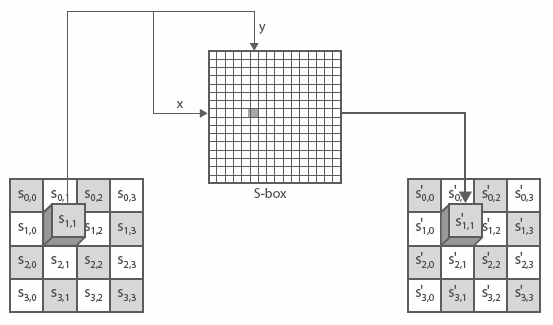
\includegraphics[scale=0.65]{assets/subbytes.png}
			      \caption{SubBytes үйлдэл}
			      \label{fig:subbytes}
		      \end{figure}
		\item \textbf{ShiftRows:}
		      \begin{itemize}
			      \item 1-р мөрийг шилжүүлэхгүй
			      \item 2–р мөрийн байтуудыг зүүн тийш 1 байт шилжүүлнэ
			      \item 3–р мөрийн байтуудыг зүүн тийш 2 байт шилжүүлнэ
			      \item 4–р мөрийн байтуудыг зүүн тийш 3 байт шилжүүлнэ
			      \item Тайлах үйлдлийг хийхдээ баруун тийш шилжүүлэх үйлдлийг хийнэ
		      \end{itemize}
		      \begin{figure}[h]
			      \centering
			      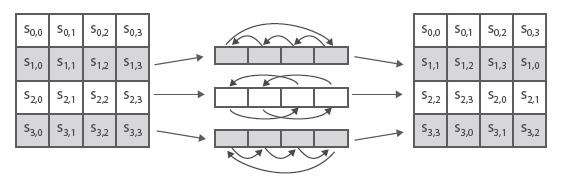
\includegraphics[scale=0.6]{assets/shiftrows.png}
			      \caption{ShiftRows үйлдэл}
			      \label{fig:shiftrows}
		      \end{figure}
		\item \textbf{MixColumns:}
		      \begin{itemize}
			      \item Багана бүр тус тусдаа холигдоно
			      \item Багана болгоны харгалзаа байтууд хоорондоо солигдоно
		      \end{itemize}
		      \begin{figure}[h]
			      \centering
			      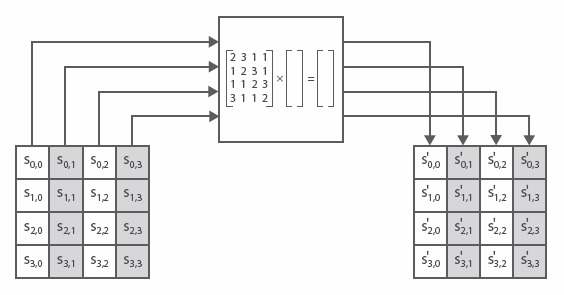
\includegraphics[scale=0.6]{assets/mixcolumns.png}
			      \caption{MixColumns үйлдэл}
			      \label{fig:mixcolumns}
		      \end{figure}
		\item \textbf{AddRoundKey:}
		      \begin{itemize}
			      \item 128 бит XOR үйлдлийг циклийн түлхүүрт ашиглана
			      \item Тайлах үйлдэл хийх бол эсрэгээр гүйцэтгэнэ
		      \end{itemize}
		      \begin{figure}[h]
			      \centering
			      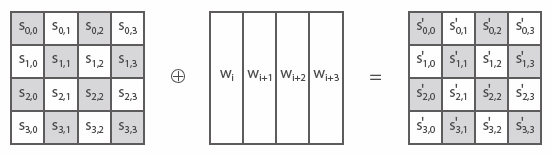
\includegraphics[scale=0.6]{assets/addroundkey.png}
			      \caption{AddRoundKey үйлдэл}
			      \label{fig:addroundkey}
		      \end{figure}
	\end{enumerate}

	\subsubsection{AES-ын нууцлалт}
	\begin{enumerate}
		\item шифрлэх блок ба түлхүүрийн урт, мөчлөгийн тоог сонгох. Шифрлэх блок ба түлхүүрийн урт нь 128, 192, 256 байт байж болох бөгөөд мөчлөгийн тоо нь харгалзан 10, 12, 14 байна.
		\item Шифрлэх текст, түлхүүрийн матриц \textit{T, W, K}-г үүсгэнэ.
		\item Эцсийн мөчлөгөөс бусад мөчлөгийн \textit{T, W, K} матрицуудад \textbf{AES}-н үндсэн үйлдлүүдийг дэс дараалан хийнэ. Харин эцсийн мөчлөгт Mix Columns үйлдлийг хийхгүй.
	\end{enumerate}
	% \subsubsection{Нууцын тайлалт}
	% 4x4 for matrix below
	\begin{center}
		$\begin{bmatrix}
				b_{0} & b_{4} & b_{8}  & b_{12} \\
				b_{1} & b_{5} & b_{9}  & b_{13} \\
				b_{2} & b_{6} & b_{10} & b_{14} \\
				b_{3} & b_{7} & b_{11} & b_{15} \\
			\end{bmatrix}$
	\end{center}
	\subsection{РСА (RSA)}
	РСА (RSA) нь анхны тооны өвөрмөц шинж чанарыг ашигладаг тэгш бус хэмтэй шифрлэлтийн арга юм. Анх 1977 онд танилцуулагдсан ба, өнөөг хүртэл хэрэглээнд хэвээр байгаа. Өнөөдрийн дэлхий даяар мөрдөгдөж байгаа стандарт нь хоёр анхны тооны үржвэр болох модулус нь 2048 бит хэмжээтэй байх ёстой. Энэ нь 617 оронтой тоо байна гэсэн үг юм.
	\begin{itemize}
		\item Хоёр анхны тоо болох $p$ болон $q$ сонгоно.
		\item $n = p*q$ утгыг олно.
		\item $\phi(n) = (p-1)*(q-1)$ утгыг олно.
		\item Дараах нөхцөлийг хангах $e$ тоог сонгоно $1 < e < \phi(n)$ ба хиех$(e, \phi(n)) = 1$.
		\item $d$ нь $d \equiv e^{-1} \mod \phi(n)$ гэж тодорхойлогдоно.
	\end{itemize}

	Нийтийн түлхүүр нь $(e, n)$ болох ба хувийн түлхүүр нь $(d, n)$ болно.\cite{РСА (RSA)}
	
\subsubsection{Нууцлал}
РСА (RSA) алгоритмын нууцлал маш том хэмжээний анхны тоог хоёр тооны үржигдэхүүн болгон задлах дээр тогтдог ба өнөөгийн бидний машины тооцон бодох чадал хараахан хангалттай биш байгаа юм.

\begin{table}[h!]
	\centering
	\caption{Муйхар хүчний алгоритм ашиглан РСА (RSA) нууцлалыг эвдэх нь \cite{Brute-force-РСА (RSA)}}
	\begin{tabular}{|c|c|c|c|}
	\hline
	n & p*q & Оролдого (Хайлт) & Хугацаа (секунд) \\
	\hline
	187 & $11 \times 17$ & 5 & $0.00344800949097$ \\
	913 & $11 \times 83$ & 5 & $0.00358390808105$ \\
	14041 & $19 \times 739$ & 8 & $0.004469871521$ \\
	557009 & $653 \times 853$ & 119 & $0.00167393684387$ \\
	9192907 & $937 \times 9811$ & 159 & $0.00201606750488$ \\
	37675201 & $3907 \times 9643$ & 540 & $0.0139532089233$ \\
	17614895377 & $40559 \times 434303$ & 4252 & $0.117401838303$ \\
	599855115407 & $694789 \times 863363$ & 56166 & $0.712327957153$ \\
	4684589242027 & $837533 \times 5593319$ & 66714 & $1.99000310898$ \\
	6833740248499 & $2565161 \times 2664059$ & 187492 & $2.51408982277$ \\
	91063247464523 & $9577907 \times 35324489$ & 188371 & $8.69724798203$ \\
	\hline
	\end{tabular}
	\end{table}

	Хамгийн сүүлд үржигдэхүүнд задалж чадсан буюу нууцлал нь амжилттай эвдэгдсэн нь РСА (RSA)-250 буюу 829 бит урттай байгаа юм. Фабрис Будот, Пьеррик Гаудри, Ауроре Гилевич, Надия Хенингер, Эммануэль Томе, Пол Циммерманн нараар ахлуулсан судлаачдын баг үүнийг 2020 онд гүйцэтгэсэн. Тооцоололд ойролцоогоор 2700 цөм жил \footnote{Цөм жил гэдэг нь CPU-ний нэг цөмийг бүтэн жил ашигласантай тэнцэнэ.} зарцуулагдсан бөгөөд шигших үе шат нь хуанлийн 35 долоо хоног янз бүрийн машинууд дээр хийгдсэн.

	\begin{figure}[h]
		\centering
		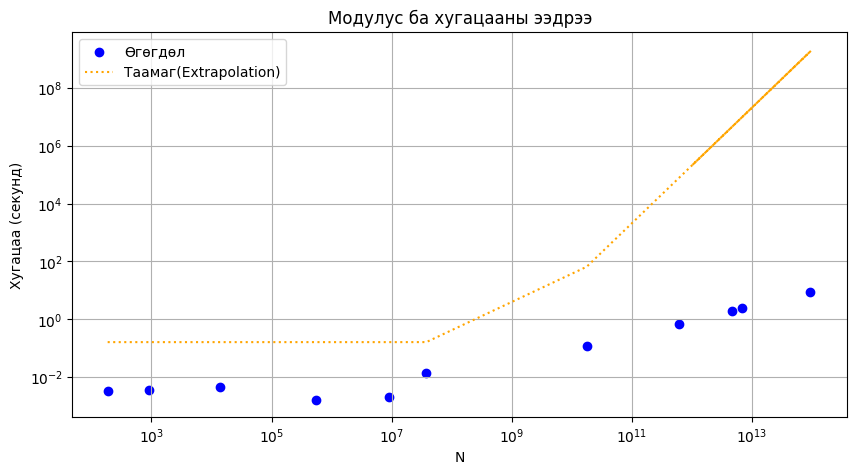
\includegraphics[scale=0.73]{assets/rsacomplexity.png}
		\caption{Хугацааны ээдрээ}
		\label{fig:rsacomplexity}
	\end{figure}

РСА (RSA) үржигдэхүүн задлах нь(factoring) цифрийн тоо нэмэгдэх тусам илтгэгч функцээр хугацааны ээдрээ тооцогдох тул одоогийн байдлаар РСА (RSA) 1024, РСА (RSA) 2048 нь хангалттай аюулгүй байгаа бөгөөд дэлхий нийтээрээ ашиглаж байна. Энэ нь дээрх диаграммаас харагдана.

\subsection{ECC (Эллипс муруйлаг криптограф)}

Эллипс муруйлаг криптографи (ECC) нь хязгаарлагдмал талбар дээрх эллипс муруйнуудын алгебрийн бүтцэд суурилсан нийтийн түлхүүрийн криптографийн нэг төрөл юм. Том бүхэл тоонуудын үржвэр дээр суурилдаг RSA-аас ялгаатай нь ECC нь эллиптик муруй дискрет логарифмын бодлогыг (ECDLP) шийдвэрлэхэд хүндрэлтэй байдгаас аюулгүй байдлаа олж авдаг. RSA-аас ECC-ийн мэдэгдэхүйц давуу тал нь түүний үр ашигтай байдал юм; ECC нь RSA-тай ижил түвшний аюулгүй байдлыг RSA-н хажууд асар жижиг хэмжээтэй түлхүүрээр олгодог. Үр ашиг нь илүү хурдан тооцоолол, эрчим хүчний бага зарцуулалт, илүү жижиг хэмжээтэй түлхүүр гэх мэт орох ба ECC нь хөдөлгөөнт төхөөрөмж, ухаалаг карт зэрэг хязгаарлагдмал нөөцтэй төхөөрөмжүүдэд илүү тохиромжтой.
\subsection{ECC ба RSA харьцуулалт}
\begin{table}[h]
	\centering
	\begin{tabular}{|c|c|c|}
	\hline
	\textbf{Битийн аюулгүй байдлын түвшин} & \textbf{RSA бит хэмжээ} & \textbf{ECC бит хэмжээ} \\ \hline
	80                          & 1024                      & 160                       \\ \hline
	112                         & 2048                      & 224                       \\ \hline
	128                         & 3072                      & 256                       \\ \hline
	192                         & 7680                      & 384                       \\ \hline
	256                         & 15360                     & 512                       \\ \hline
	\end{tabular}
	\caption{Аюулгүй байдлын түвшин ба RSA болон ECC түлхүүрийн хэмжээг харьцуулах \cite{RSAvsECC}}
	\label{tab:rsa_ecc_key_sizes}
	\end{table}
	
	\begin{figure}[h]
		\centering
		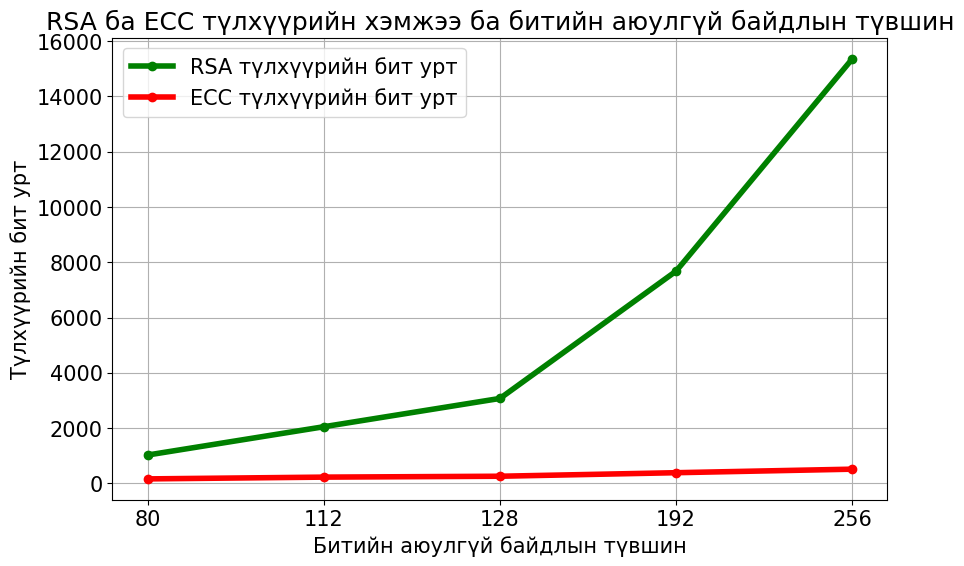
\includegraphics[scale=0.6]{assets/graphs/keysize.png}
		\caption{RSA ба ECC түлхүүрийн хэмжээнүүдийн харьцуулалт}
		\label{fig:architecture}
	\end{figure}
	\begin{figure}[h]
		\centering
		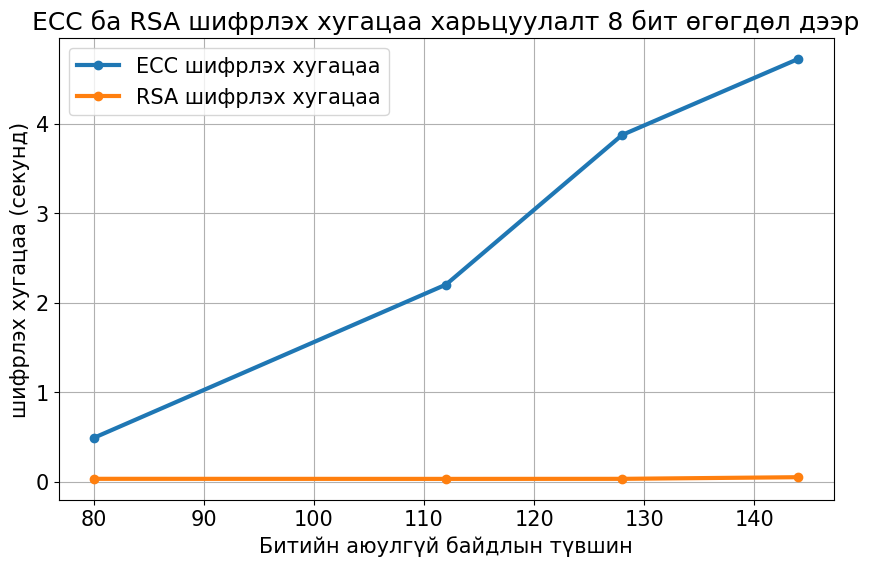
\includegraphics[scale=0.65]{assets/graphs/1.png}
		\caption{8 бит өгөгдөл шифрлэлт}
		\label{fig:architecture}
	\end{figure}
	\begin{figure}[h]
		\centering
		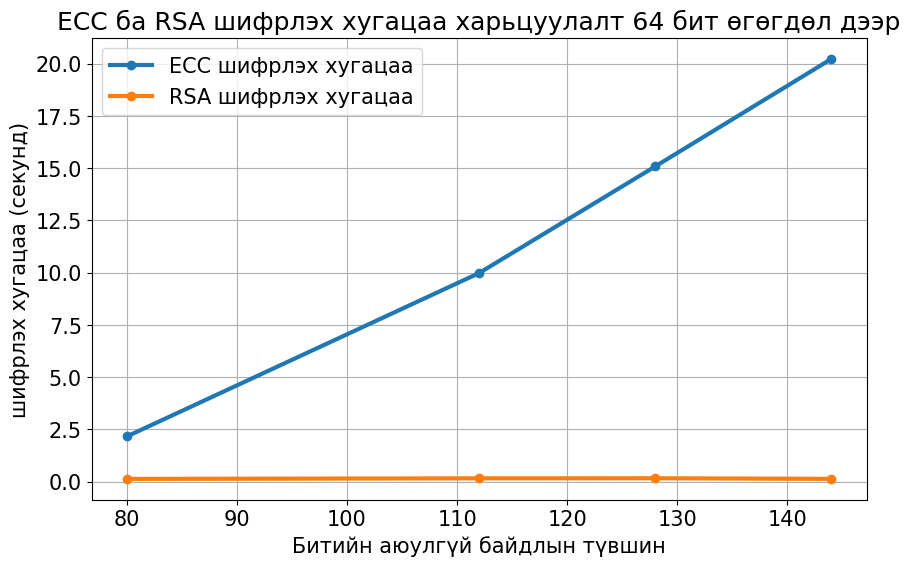
\includegraphics[scale=0.65]{assets/graphs/2.png}
		\caption{64 бит өгөгдөл шифрлэлт}
		\label{fig:architecture}
	\end{figure}
	\begin{figure}[h]
		\centering
		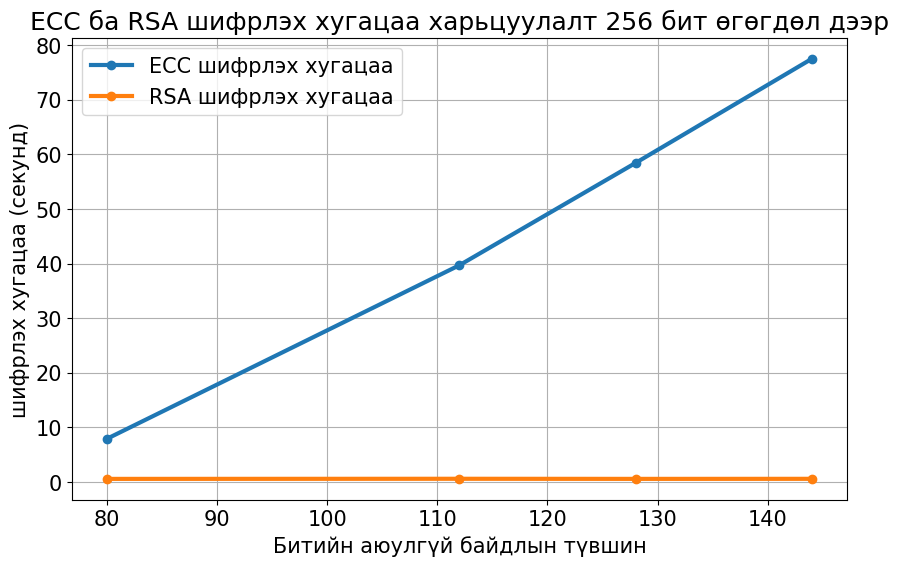
\includegraphics[scale=0.65]{assets/graphs/3.png}
		\caption{256 бит өгөгдөл шифрлэлт}
		\label{fig:architecture}
	\end{figure}
	\begin{figure}[h]
		\centering
		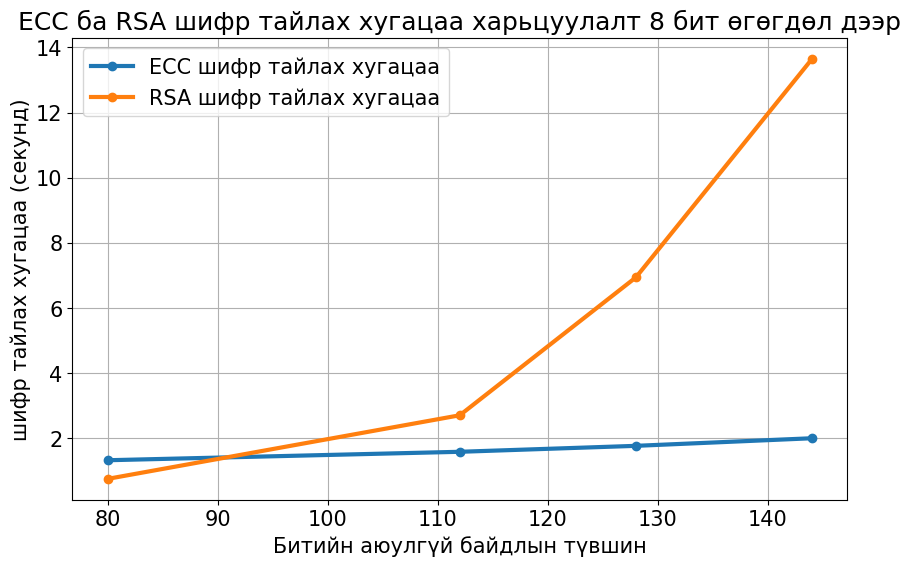
\includegraphics[scale=0.65]{assets/graphs/4.png}
		\caption{8 бит өгөгдөл шифрлэлт тайлалт}
		\label{fig:architecture}
	\end{figure}
	\begin{figure}[h]
		\centering
		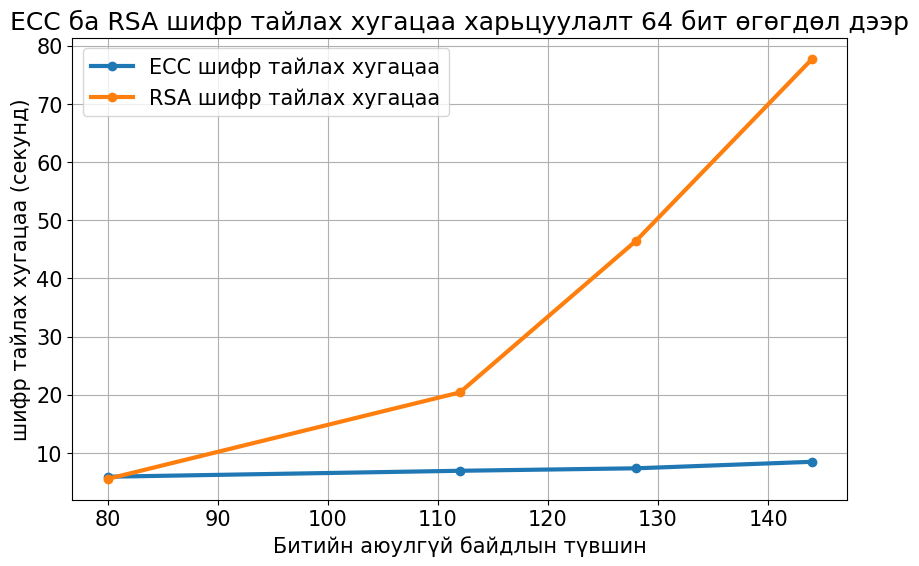
\includegraphics[scale=0.65]{assets/graphs/5.png}
		\caption{64 бит өгөгдөл шифрлэлт тайлалт}
		\label{fig:architecture}
	\end{figure}
	\begin{figure}[h]
		\centering
		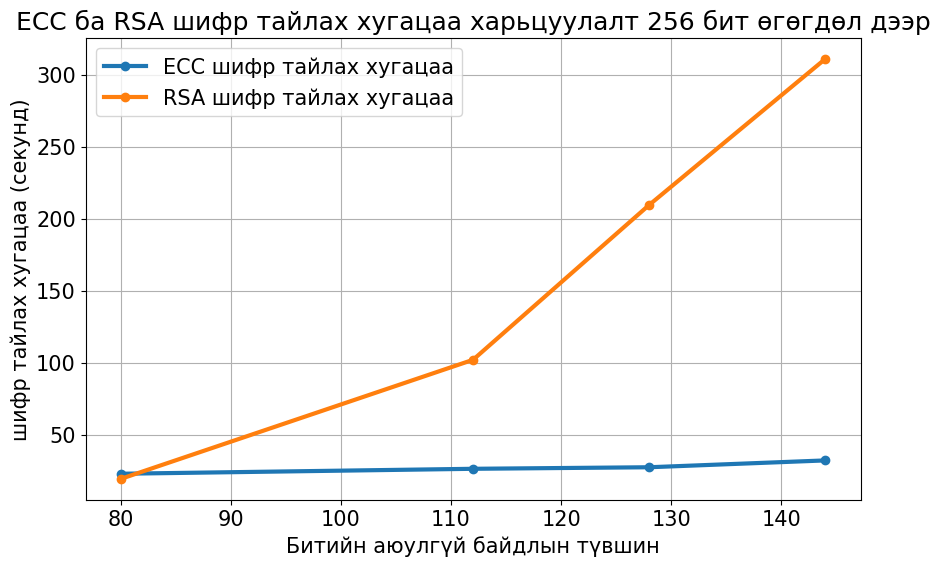
\includegraphics[scale=0.65]{assets/graphs/6.png}
		\caption{256 бит өгөгдөл шифрлэлт тайлалт}
		\label{fig:architecture}
	\end{figure}
	\begin{figure}[h]
		\centering
		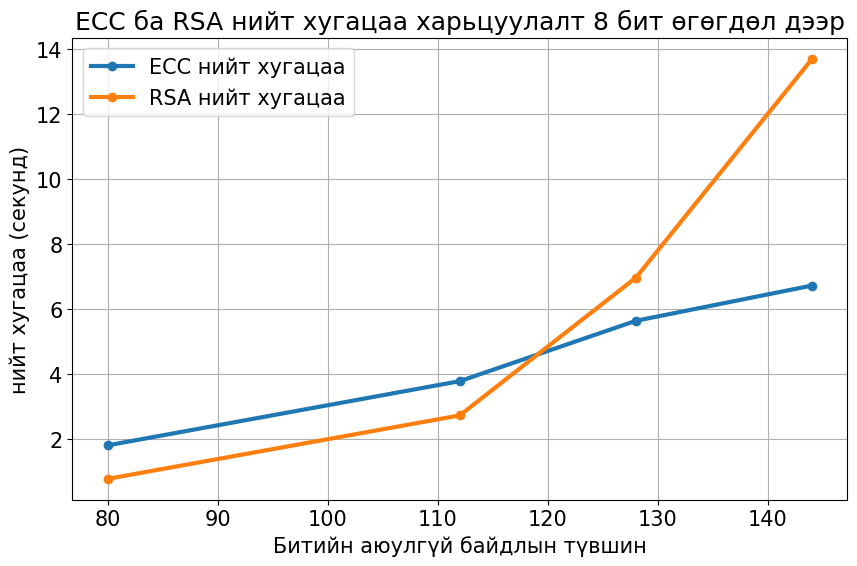
\includegraphics[scale=0.65]{assets/graphs/7.png}
		\caption{8 бит өгөгдөл хугацааны харьцуулалт}
		\label{fig:architecture}
	\end{figure}
	\begin{figure}[h]
		\centering
		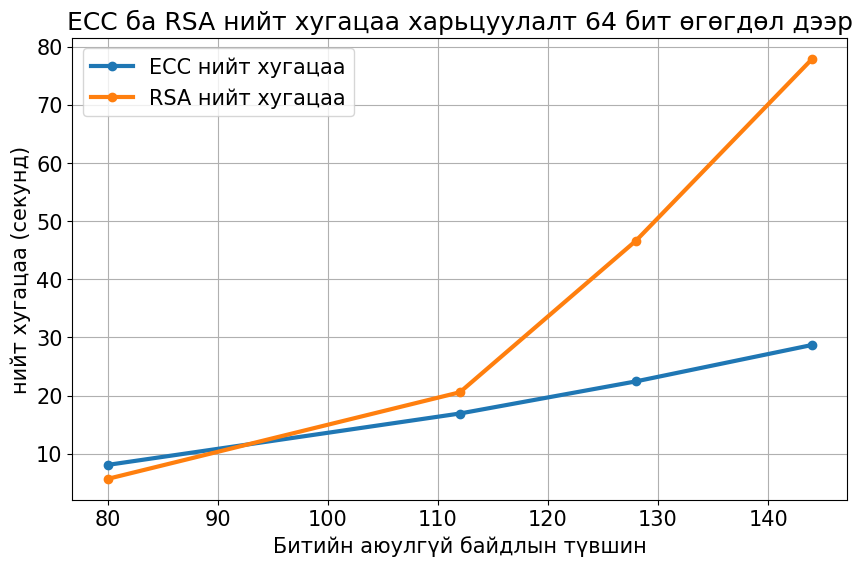
\includegraphics[scale=0.65]{assets/graphs/8.png}
		\caption{64 бит өгөгдөл хугацааны харьцуулалт}
		\label{fig:architecture}
	\end{figure}
	\begin{figure}[h]
		\centering
		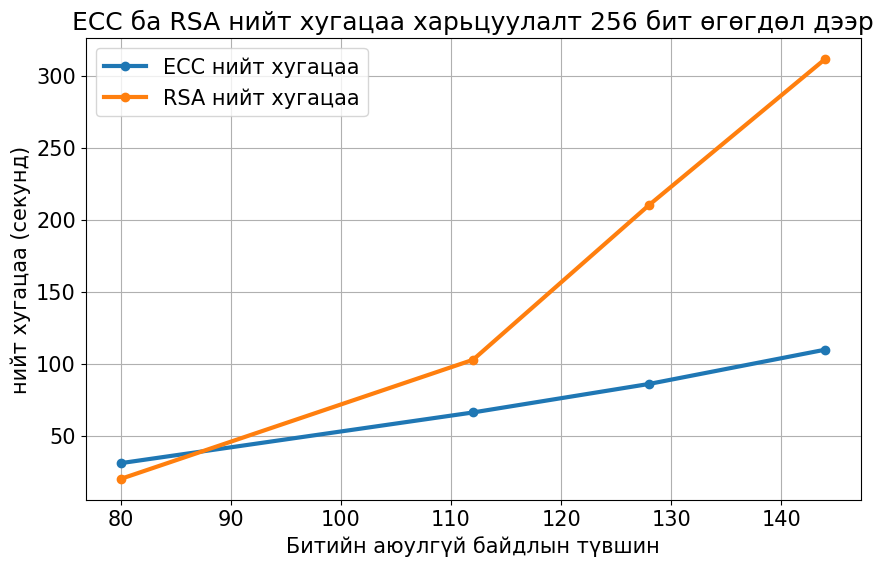
\includegraphics[scale=0.65]{assets/graphs/9.png}
		\caption{256 бит өгөгдөл хугацааны харьцуулалт}
		\label{fig:architecture}
	\end{figure}
	
	
	\begin{table}
	\centering
	\caption{8 бит өгөгдөл – шифрлэлт ба шифр тайлах хугацаа (Секундээр) \cite{RSAvsECC}}
	\begin{tabular}{|c|c|c|c|c|c|c|}
	\hline
	Хамгаалалт & ECC шифр & RSA шифр & ECC тайлах & RSA тайлах & ECC & RSA \\
	\hline
	80 & 0.4885 & 0.0307 & 1.3267 & 0.7543 & 1.8152 & 0.7850 \\
	112 & 2.2030 & 0.0299 & 1.5863 & 2.7075 & 3.7893 & 2.7375 \\
	128 & 3.8763 & 0.0305 & 1.7690 & 6.9409 & 5.6453 & 6.9714 \\
	144 & 4.7266 & 0.0489 & 2.0022 & 13.6472 & 6.7288 & 13.6962 \\
	\hline
	\end{tabular}
	\end{table}
	
	\begin{table}
	\centering
	\caption{64 бит өгөгдөл – шифрлэлт ба шифр тайлах хугацаа (Секундээр) \cite{RSAvsECC}}
	\begin{tabular}{|c|c|c|c|c|c|c|}
	\hline
	Хамгаалалт & ECC шифр & RSA шифр & ECC тайлах & RSA тайлах & ECC  & RSA  \\
	\hline
	80 & 2.1685 & 0.1366 & 5.9099 & 5.5372 & 8.0784 & 5.6738 \\
	112 & 9.9855 & 0.1635 & 6.9333 & 20.4108 & 16.9188 & 20.5743 \\
	128 & 15.0882 & 0.1672 & 7.3584 & 46.4782 & 22.4466 & 46.6454 \\
	144 & 20.2308 & 0.1385 & 8.4785 & 77.7642 & 28.7093 & 77.9027 \\
	\hline
	\end{tabular}
	\end{table}
	
	\begin{table}
	\centering
	\caption{256 бит өгөгдөл – шифрлэлт ба шифр тайлах хугацаа (Секундээр) \cite{RSAvsECC}}
	\begin{tabular}{|c|c|c|c|c|c|c|}
	\hline
	Хамгаалалт & ECC шифр & RSA шифр & ECC тайлах & RSA тайлах & ECC  & RSA  \\
	\hline
	80 & 7.9240 & 0.5596 & 22.8851 & 19.3177 & 30.8091 & 19.8772 \\
	112 & 39.7008 & 0.5815 & 26.3331 & 102.0337 & 66.0339 & 102.6153 \\
	128 & 58.4386 & 0.5611 & 27.4060 & 209.6086 & 85.8446 & 210.1697 \\
	144 & 77.5034 & 0.5718 & 32.1522 & 311.0649 & 109.6556 & 311.6368 \\
	\hline
	\end{tabular}
	\end{table}
	